% chktex-file 44
\chapter[Detection of Planetary Emission from TrES-2 using \emph{Spitzer}/ IRAC]
{%
Detection of Planetary Emission from TrES-2 using \emph{Spitzer}/IRAC%
\protect\CFNE%
}\label{cha:spitzer}

\section*{Abstract}\label{cha:spitzer:sec:abs}
\addcontentsline{toc}{section}{Abstract}

With the discovery of nine new transiting planets within the last year, there have been ample candidates for Target of Opportunity observations using the {\textit Spitzer Space Telescope}.
We present here the results of the first of two planned series of observations of \tresTwo\ using the Infrared Array Camera on \spi.
\tresTwo\ is the most massive such candidate to be observed with \spi.
The brightness of this transiting system is seen to decrease by \mbox{$0.168 \pm 0.022$\,\%} at 4.5\,$\mu$m, and \mbox{$0.253 \pm 0.045$\,\%} at 8.0\,$\mu$m, during the secondary eclipse when the planetary emission is blocked by the star.
We show that these flux contrasts are well fit by a blackbody spectrum (similar to the results from recent infrared observations of transiting hot Jupiters) with \mbox{$T_{\mathrm eff}=1450$\,K}, as well as by a more detailed model spectrum with a planetary $T_{\mathrm eff}$ of 1550\,K and near-uniform redistribution of the stellar insolation.
The time of the center of the secondary eclipse of \tresTwo\ is found to be consistent with predictions based on recent observations of transits of \tresTwo.
This implies that \tresTwo\ mostly likely has a circular orbit, and thus does not obtain additional thermal energy from tidal dissipation of a nonzero orbital eccentricity.

\section[\textit{Spitzer} Observations of the Known Transiting Exoplanets]{\textbf{\textit{Spitzer}} Observations of the Known Transiting Exoplanets}\label{cha:spitzer:sec:intro}

There has been a recent dramatic increase in the number of nearby ($d<300$\,pc) extrasolar planets whose structures and atmospheric compositions can be probed using the {\textit Spitzer Space Telescope}.
These are the nearby transiting exoplanets (14 at the time of writing, 10 of which were discovered in the last year).
{\textit Spitzer} observations of these planets will help us understand the thermal dynamics associated with the high insolation onto these planetary atmospheres, and thus how the radius of a hot Jupiter varies with its mass.

Although over 200 extrasolar planets are known, it is only for these 14 nearby transiting exoplanets that we can measure the planetary radius and true planetary mass precisely enough to provide tight constraints for theoretical models.
There have been problems reconciling the observed planetary mass and radius with models (\citealp[see][for a review]{Laughlin_Wolf_Vanmunster:apj:2005a, Charbonneau_Brown_Burrows:PPV:2007a}).
Several explanations have been proposed for the bloated planets, mainly regarding some additional source of energy combating planetary contraction (\citealp[see, e.g.,][]{Guillot_Showman:aa:2002a}). \citet{Deming_Seager_Richardson:nat:2005a} refuted the possibility that tidal damping of a nonzero eccentricity was one such energy source for \hdTZNb\ (Bodenheimer, Lin, \& Mardling~\citeyear{Bodenheimer_Lin_Mardling:apj:2001a}; Bodenheimer, Laughlin, \& Lin~\citeyear{Bodenheimer_Laughlin_Lin:apj:2003a}).
By measuring the timing of the secondary eclipse of \hdTZNb, they showed that the planetary orbit is circular, as expected for a hot Jupiter, unless it is gravitationally affected by an unseen planetary companion (\citealp[see, e.g.,][]{Rasio_Ford:Science:1996a}).
In order to fully understand these inflated radii, we have begun to estimate the atmospheric composition of the nearby exoplanets (\citealp[for a discussion of extrasolar planetary atmospheres, see][]{Charbonneau_Brown_Burrows:PPV:2007a, Marley_Fortney_Seager:PPV:2007a}).
Detection of \emph{emission} from planetary atmospheres was made possible by taking advantage of the enhanced contrast between stars and their planets in the infrared.
Infrared emission has been detected from \hdTZNb\ and \hdOENb, both at specific wavelengths \citep{Deming_Seager_Richardson:nat:2005a, Deming_Harrington_Seager:apj:2006a}, and over a wide spectral range \citep{Richardson_Deming_Horning:Nature:2007a, Swain_Bouwman_Akeson:preprint:2007a, Grillmair_Charbonneau_Burrows:apjl:2007a}.
\citet{Charbonneau_Allen_Megeath:apj:2005a} also reported infrared emission from \tresOne.
There has been a flurry of activity to reconcile atmospheric models with this limited number of infrared measurements.
While several attempts have been made to explain the infrared observations (\citealp[see, e.g.,][]{Barman_Hauschildt_Allard:apj:2005a}; \citealp*{Burrows_Hubeny_Sudarsky:apjl:2005a}; \citealp{Burrows_Hubeny_Budaj:apj:2007a}; \citealp{Fortney_Marley_Lodders:apjl:2005a}; \citealp{Fortney_Cooper_Showman:apj:2006a}; \citealp{Seager_Richardson_Hansen:apj:2005a}), the models are not entirely in agreement and no single model can explain every observation.
There is a clear need to obtain as many additional observations of extrasolar planetary atmospheres as possible during \spi's limited lifetime.

The transiting hot Jupiter \tresTwo\ (\citealp{ODonovan_Charbonneau_Mandushev:apjl:2006a}, see chapter~\ref{cha:tres2}) is the most massive of the transiting systems that has been followed up with \spi, providing a key constraint for our understanding of the gas giant mass-radius relation.
Here we present the first \spi\ observations of \tresTwo\ (section~\ref{cha:spitzer:sec:obs}).
From our analysis (section~\ref{cha:spitzer:sec:lc}), we have detected thermal emission from the transiting planet, and compared our results with various atmospheric models (section~\ref{cha:spitzer:sec:atm}).

\section{IRAC Observations of TrES-2}\label{cha:spitzer:sec:obs}

In a similar manner to the previous \spi\ observations of \tresOne\ (Charbonneau et al., \citeyear{Charbonneau_Allen_Megeath:apj:2005a}), we employed two of the four bandpasses available on the Infrared Array Camera (IRAC; \citealt{Fazio_Hora_Allen:apjs:2004a}) on \spi\ to monitor \tresTwo\ during the time of secondary eclipse.
We selected the 4.5-$\mu$m and 8.0-$\mu$m channels; future observations of \tresTwo\ at 3.6\,$\mu$m and 5.8\,$\mu$m are planned.
We took care to position \tresTwo\ (\tresTwoTwoMass: \mbox{$J=10.232$\,mag}, \mbox{$J-K_{s}=0.386$\,mag}) away from array regions impaired by bad pixels or scattered light.
We also kept the corresponding IRAC stray light avoidance zones free of stars that are bright in the infrared.
We observed a \mbox{$5\farcm2 \times 5\farcm2$} field of view (FOV) containing \tresTwo\ for 3.9\,hr on UT 2006 November~30 (starting at \mbox{$\mathrm{HJD}\,2,\!454,\!069.956$}), and obtained 1073 images in both channels with an effective integration time of 10.4\,s.

\section[Deriving and Modeling Light Curves of TrES-2]{Deriving and Modeling Light Curves of \\ TrES-2}\label{cha:spitzer:sec:lc}

As part of the standard pipeline for IRAC data, the images are dark current subtracted, flat-fielded, and corrected for any detector nonlinearity.
Each header of these Basic Calibrated Data (BCD) images contains the time and date of observation and the effective integration time.
We used these to compute the Julian date corresponding to mid-exposure of each observation.
In order to convert these dates to Heliocentric Julian dates, we subtracted 30.926\,s from each to account for the light travel time between the Sun and \spi.
We then computed the orbital phases using the orbital period (\mbox{$P=2.47063\pm0.00001$\,days}) from \citeauthor{ODonovan_Charbonneau_Mandushev:apjl:2006a}~(\citeyear{ODonovan_Charbonneau_Mandushev:apjl:2006a}, see chapter~\ref{cha:tres2}) and an updated transit epoch (\mbox{$T_{C} = \mathrm{HJD}~2,\!454,\!041.63598\pm0.00030$}; \citealt{Holman_Winn_Latham:apj:2007a}) derived from recent observations made as part of the Transit Light Curve project.

Using an initial estimate of the position of \tresTwo\ on the array, we computed the arithmetic centroid of \tresTwo\ in each BCD image.
We then measured the flux from our target using circular apertures ranging from 2 to 10 pixels, and sky subtracted using a sky annulus with inner and outer radii of 20 and 30 pixels, respectively.
We normalized the fluxes for a given channel and aperture size using the corresponding median flux value.
We examined the variation of the rms of the out-of-eclipse data, and found that an aperture size of 3 pixels produced the smallest rms for both channels.
We then performed a separate analysis of these two light curves from the two channels, as IRAC displays different characteristics at 4.5\,$\mu$m and 8.0\,$\mu$m.

\begin{figure}
\begin{center}
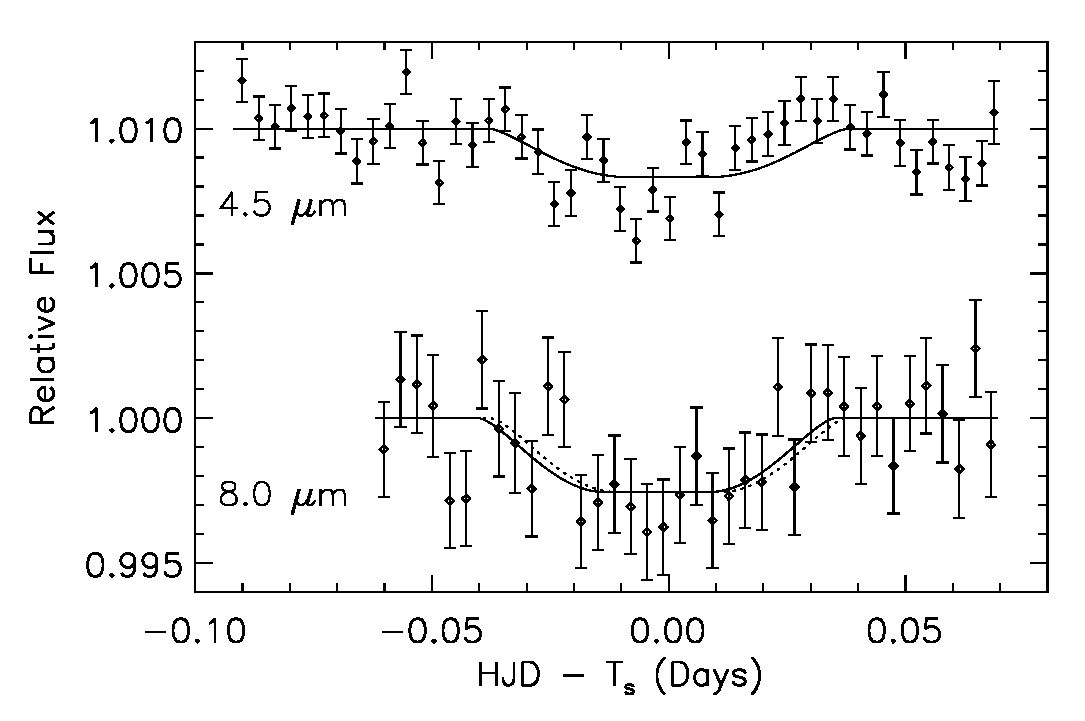
\includegraphics[width=0.95\textwidth]{6_f1}
\caption[%
Near-infrared relative fluxes from TrES-2 from {\textit Spitzer} observations]{%
Relative fluxes from the TrES-2 system at 8.0\,$\mu$m ({\textit bottom}) and at 4.5\,$\mu$m ({\textit top}, with an arbitrary flux offset), binned and plotted versus the time from the predicted center of secondary eclipse ($T_{s}$).
Superimposed are our best-fit models (\emph{black lines}) with depths of \mbox{$\Delta f_{\mathrm {4.5}} = 0.00168 \pm 0.00022$} and \mbox{$\Delta f_{\mathrm {8.0}} = 0.00253 \pm 0.00045$}, respectively.
The timing of the secondary eclipse was allowed to vary for the 8.0-$\mu$m data (but not for the 4.5-$\mu$m data), and the derived timing offset (\mbox{$\Delta t_{\mathrm {8.0}} = -3.6^{+5.8}_{-4.4}$\,minutes}) is consistent with eclipse occurring at the predicted $T_{s}$.
The \emph{dotted line} represents a model with the same depth as our best-fit model of the 8.0-$\mu$m data, but with zero timing offset.%
}\label{cha:spitzer:fig:tres2_combplot}
\end{center}
\end{figure}

The 8.0-$\mu$m data showed an overall increase in flux with time, but the first 32 minutes of data displayed a steeper slope.
We excluded this initial data and large flux outliers from further analysis.
In order to remove the trend, we computed a linear fit to the out-of-eclipse data, and then divided the data set by this model.
In order to extract the depth and epoch of the secondary eclipse, we created a model using the eclipse light curve code for a uniform source from \citet{Mandel_Agol:apjl:2002a}, allowing the eclipse depth ($\Delta f_{\mathrm {8.0}}$) and the offset ($\Delta t_{\mathrm {8.0}} $) from the predicted eclipse epoch (\mbox{$\mathrm{HJD}\,2,\!454,\!070.04823\pm0.00030$}) to vary.
The required system parameters were the planetary orbital period, impact parameter and orbital inclination (\mbox{$P=2.47063$\,days}, \mbox{$b=0.84$}; \citealt{ODonovan_Charbonneau_Mandushev:apjl:2006a} [see chapter~\ref{cha:tres2}], and \mbox{$i=83.9\degr$} \citealt{Holman_Winn_Latham:apj:2007a}), and the radius ratio between the planet and the star (\mbox{$R_{\mathrm p}/R_{\star}=0.1251$};  \citealt{Holman_Winn_Latham:apj:2007a}).
For each pair ($\Delta f_{\mathrm {8.0}}$, $\Delta t_{\mathrm {8.0}}$) over the range($0.0005 \le \Delta f_{\mathrm 8.0} \le 0.0040$, $-40\,\mathrm{minutes} \le \Delta t_{\mathrm {8.0}} \le 40\,\mathrm{minutes}$), we computed the $\chi^{2}$ of the corresponding model to the 8.0-$\mu$m data, again excluding large flux outliers.
The best-fit values were an eclipse depth of $\Delta f_{\mathrm {8.0}} = 0.00253 \pm 0.00045$ and a timing offset of $\Delta t_{\mathrm {8.0}} = -3.6^{+5.8}_{-4.4}$\,minutes, where the negative sign in time corresponds to an early secondary eclipse.
Thus we see that the best-fit timing offset is consistent with the predicted epoch for the secondary eclipse.
Figure~\ref{cha:spitzer:fig:tres2_combplot} shows this best-fit model, superimposed with the 8.0-$\mu$m data binned using 7-minute bins.
The reduced $\chi^{2}$ for this fit was:
\begin{eqnarray*}
\chi_{\mathrm r}^{2} & = & \chi^{2}/(N-2), \\
 & = & 857.4/(852-2), \\
 & = & 1.01,
\end{eqnarray*}
corresponding to a well-fit data set.

An upper limit for the orbital eccentricity of a transiting planet can be computed from the timing offset $\Delta t_{\mathrm {8.0}}$ derived above, using $e \, \cos{\omega} \simeq \pi \, \Delta t_{\mathrm 8.0}/2 \, P$, where $\omega$ is the unknown longitude of periastron and $P$ is the known orbital period (\citealp[see equation~4 of][]{Charbonneau_Allen_Megeath:apj:2005a}).
This upper limit for \tresTwo\ is therefore \mbox{$0.00145\pm0.00096$}, consistent with a negligible orbital eccentricity.
Spitzer has also obtained a negligible orbital eccentricity for two other planets: \hdTZNb\ \citep{Deming_Seager_Richardson:nat:2005a} and \tresOne\ \citep{Charbonneau_Allen_Megeath:apj:2005a}.
Tidal damping of orbital eccentricity (Bodenheimer, Lin, \& Mardling~\citeyear{Bodenheimer_Lin_Mardling:apj:2001a}; Bodenheimer, Laughlin, \& Lin~\citeyear{Bodenheimer_Laughlin_Lin:apj:2003a} has yet to be shown to be a sizable contribution to the internal energy of any exoplanet.

The analysis of the 4.5-$\mu$m data was complicated by the known correlation between the IRAC 4.5-$\mu$m flux from a source and the intra-pixel position on the detector.
For this data set, we assumed the eclipse occurred at the predicted time (consistent with the above 8.0-$\mu$m timing offset for this secondary eclipse), and measured the eclipse depth at this wavelength.
Here we excluded outliers not only in flux, but also in $x$ or $y$ position.
Our model consisted of the product of a model eclipse light curve
and a second-order polynomial in $x$ and $y$.
Again, we minimized the $\chi^{2}$ of our model fit to the 4.5-$\mu$m data, this time using the AMOEBA algorithm \citep{Press_Teukolsky_Vetterling:1992a}.
The derived 4.5-$\mu$m eclipse depth was \mbox{$\Delta f_{\mathrm {4.5}} = 0.00168 \pm 0.00022$}.
The reduced $\chi^{2}$ for this fit was \mbox{$\chi_{\mathrm r}^{2} = 798.8/(1051-1)=0.76$}, corresponding to a well-fit data set.
In figure~\ref{cha:spitzer:fig:tres2_combplot}, we show our binned 4.5-$\mu$m data, together with our best-fit theoretical light curve.

\section{Atmospheric Models for TrES-2}\label{cha:spitzer:sec:atm}

\begin{figure}
\begin{center}
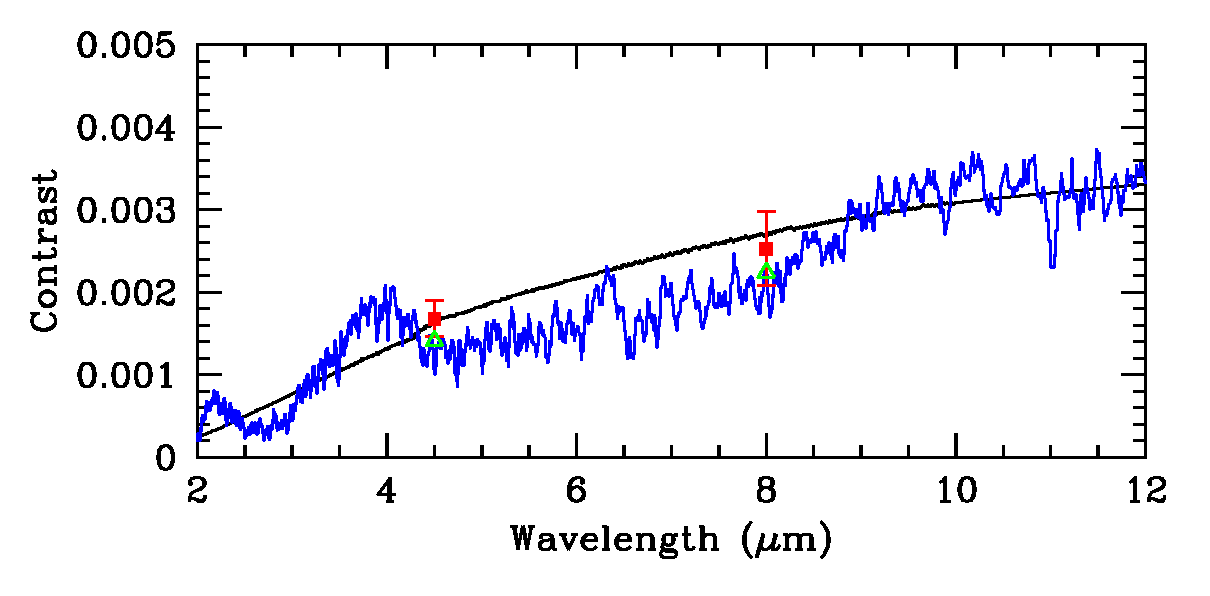
\includegraphics[width=0.95\textwidth]{6_f2}
\caption[%
Near-infrared contrast ratios for TrES-2]{%
Contrast ratios ({\textit red squares}) for TrES-2 at 4.5\,$\mu$m and 8.0\,$\mu$m, which are consistent with a model ({\textit black line}) of a 1450\,K blackbody planetary flux divided by a Kurucz model of the star TrES-2. Also shown are the predictions ({\textit green triangles}) for these fluxes from a theoretical planet-star flux contrast model ({\textit blue line}) computed for the star TrES-2 using the \citet{Seager_Richardson_Hansen:apj:2005a} code (see text).%
}\label{cha:spitzer:fig:tres2models}
\end{center}
\end{figure}

We now turn to a discussion of the \tresTwo\ 4.5-$\mu$m and 8.0-$\mu$m planet-star contrast.
We first emphasize how well the data are fit by a blackbody spectrum of 1450\,K.
The {\textit black line} in figure~\ref{cha:spitzer:fig:tres2models} is a 1450\,K blackbody flux divided by a Kurucz stellar model appropriate for the stellar parameters derived by \citet{Sozzetti_Torres_Charbonneau:apj:2007a}.
A blackbody of 1450\,K implies a Bond albedo of 0.12, with the assumption of uniform redistribution of absorbed stellar radiation.
If \tresTwo\ is indeed a blackbody, it would add to the growing list of published hot Jupiter atmosphere data commensurate with blackbody spectra, showing no evidence for the atmospheric composition.
These exoplanets include two of the three exoplanets with more than one published data point: \tresOne\ \citep{Charbonneau_Allen_Megeath:apj:2005a} and the \hdOENb\ spectrum \citep{Grillmair_Charbonneau_Burrows:apjl:2007a}.
A theoretical planet-star flux contrast that fits the data is also shown as the {\textit blue line} in figure~\ref{cha:spitzer:fig:tres2models}.
The \tresTwo\ spectrum was generated from a model atmosphere code for hot Jupiters \citep{Seager_Richardson_Hansen:apj:2005a} with inputs appropriate to the \tresTwo\ planet-star parameters, solar abundances, and a Kurucz model atmosphere for the irradiation from the parent star.
We reduce the incident stellar flux by \mbox{$f=0.9$} to take into account the redistribution of absorbed stellar radiation.
This value is intermediate between the values for instantaneous reradiation (\mbox{$f=3/8$}) and uniform redistribution (\mbox{$f=1$}) of absorbed stellar radiation.
The planet spectrum has \mbox{$T_{\mathrm eff}=1550$\,K}.
Planets with higher values of $f$ (i.e., under the assumption that the absorbed stellar radiation is redistributed more uniformly) than the one we chose have flux values too low in both the 4.5-$\mu$m and 8.0-$\mu$m bandpasses.
We justify our somewhat arbitrary choice of $f$ based on the results of \citet{Fortney_Cooper_Showman:apj:2006a} that 1-D models do not represent the 3-D dayside temperature pressure profiles that likely result from a highly complex atmospheric circulation.

\section[Searching for Evidence of Atmospheric Absorption]{Searching for Evidence of Atmospheric \\ Absorption}\label{cha:spitzer:sec:discuss}

The \spi\ data we report for \tresTwo\ is markedly different than for \tresOne\ \\ \citep{Charbonneau_Allen_Megeath:apj:2005a}.
In comparing the \tresTwo\ and \tresOne\ data sets with each other and with models, it is useful to define a \spi\ IRAC color index: the ratio of the 8.0-$\mu$m to 4.5-$\mu$m planet-star flux contrast.
For \tresOne\ the color index is \mbox{$3.41 \pm 0.87$}.
This ratio was too high to fit most atmosphere models in the literature (\citealp[see][]{Fortney_Marley_Lodders:apjl:2005a, Seager_Richardson_Hansen:apj:2005a, Barman_Hauschildt_Allard:apj:2005a};  but cf \citealt*{Burrows_Sudarsky_Hubeny:apj:2006a}).
Although many different models (including such effects as high metallicity, energy deposition at high altitudes in the atmosphere; varying C/O ratios, energy redistribution parameterizations) have since been explored (\citealp{Barman_Hauschildt_Allard:apj:2005a}; \citealp{Fortney_Marley_Lodders:apjl:2005a}; \citealp{Seager_Richardson_Hansen:apj:2005a};  Burrows, Sudarsky, \& Hubeny \citeyear{Burrows_Sudarsky_Hubeny:apj:2006a}), none reach the \tresOne\ value of 3.4.

\tresTwo\ has a much lower color index (\mbox{$1.51 \pm 0.33$}) than \tresOne.
This value is much more easily fit by ``generic'' hot Jupiter atmosphere models.
Indeed, a wide variety of theoretical models with solar abundances, with uniform or hemispheric redistribution, with or without clouds, and for a wide range of temperatures and redistribution values, have ratios consistent with the \tresTwo\ color index \citep[see, e.g.,][]{Fortney_Marley_Lodders:apjl:2005a, Barman_Hauschildt_Allard:apj:2005a, Charbonneau_Allen_Megeath:apj:2005a}.
This is primarily because the water vapor absorption features in these models dominate the spectra, and appears to create a somewhat consistent color index.

\spi\ IRAC data at 3.6\,$\mu$m and 5.8\,$\mu$m are forthcoming for \tresTwo.
These additional data are critical to distinguish between a blackbody spectrum, a radiative equilibrium solar abundance spectrum, and other atmosphere models.
